%Name: Template of COMP9020 Assignments
%Author:Jack
%Date: 14/08/2017
%Acknowledgement: This template is based on work of Brendan Trinh of UNSW MathSoc 2015
\documentclass[11pt, a4paper]{article}

\usepackage{amsmath} % Improves structure of typed out maths
\usepackage{mathtools} % Improves upon deficiencies of amsmath package
\usepackage{amssymb} % Adds some handy symbols to use.
\usepackage{amsthm} % Adds some neat formulas to use, e.g. \begin{proof} etc.

\usepackage[a4paper]{geometry} % Default page margins can be altered.
\usepackage{microtype} % Improves spacing between letters.
\usepackage{booktabs} % Improves tables. Can now create without vertical separators.
\usepackage{array} % Includes more options for arrays
\usepackage{paralist} % More flexible use of itemize, enumerate, etc.
\usepackage{graphicx} % Add images to your document
\usepackage{color} % Allows for the use of colours!
\usepackage{cleveref} % Better cross-referencing
\usepackage{hyperref} % For adding hyperlinks
\usepackage{fancyhdr} % Customise headers & footers in document
\usepackage{paralist}

\usepackage{url} % For adding url

\begin{document}
\title{COMP9020 - Assignment 2}
\author{Jack Jiang (z5129432)}
\date{ 24 September 2017 }
\maketitle
\graphicspath{{Graphics/}}

\section*{Question 1}
\begin{enumerate}[(a)]
    \item
    For graph G = (E, V) as follows:\\
    \begin{center}
        \includegraphics{q1a1}
    \end{center}
    For every $e = (v, w) \in E$\\
    $$ c(v) \ne c(w) $$
    The mininum number of colors to sufficient effect such a mapping, denoted:
    $$ \chi(G) $$
    \item
    The minimum number of colors is 2, as follows:\\
    \begin{center}
        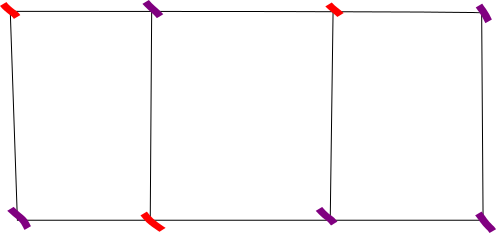
\includegraphics[scale=0.7]{q1b1}
    \end{center}
    \item
    The connection of the graph changes, as follows:\\
    \begin{center}
        \includegraphics[scale=0.7]{q1c1}
    \end{center}
    Because v2 connect to v3, so they must be different colours, $c(v2) \ne c(v3)$
    v2 and v3 connect to all other vertex, so other vertex must use different colours other than c(v2) and c(v3)
    $$c(v1) \ne c(v2) \ne c(v3)$$
    also, v1 connect to v4, so $c(v1) \ne c(v4)$, at lease we should use 4 different colors
    Because I can use 4 different colors as shows in graph, therefore:
    $$ \chi(G) = 4 $$
\end{enumerate}

\section*{Question 2}
\begin{enumerate}[(a)]
    \item


    \item


    \item


\end{enumerate}



\end{document}